\documentclass[11pt]{article}
\usepackage[utf8]{inputenc}
\usepackage{verbatim}
\usepackage{subfig}
\usepackage{makeidx}
\usepackage{listings}
\usepackage{color}
\usepackage{tikz}
\usetikzlibrary{arrows}
\usepackage{pgf}
\usepackage{fancybox}
\usepackage{verbatim}
\usepackage{wrapfig}

\definecolor{dkgreen}{rgb}{0,0.6,0}
\definecolor{gray}{rgb}{0.5,0.5,0.5}
\definecolor{mauve}{rgb}{0.58,0,0.82}

\lstset{ %
  language=Octave,                % the language of the code
  basicstyle=\footnotesize,           % the size of the fonts that are used for the code
  numbers=left,                   % where to put the line-numbers
  numberstyle=\tiny\color{gray},  % the style that is used for the line-numbers
  stepnumber=2,                   % the step between two line-numbers. If it's 1, each line
  % will be numbered
  numbersep=5pt,                  % how far the line-numbers are from the code
  backgroundcolor=\color{white},      % choose the background color. You must add \usepackage{color}
  showspaces=false,               % show spaces adding particular underscores
  showstringspaces=false,         % underline spaces within strings
  showtabs=false,                 % show tabs within strings adding particular underscores
  frame=single,                   % adds a frame around the code
  rulecolor=\color{black},        % if not set, the frame-color may be changed on line-breaks within not-black text (e.g. commens (green here))
  tabsize=2,                      % sets default tabsize to 2 spaces
  captionpos=b,                   % sets the caption-position to bottom
  breaklines=true,                % sets automatic line breaking
  breakatwhitespace=false,        % sets if automatic breaks should only happen at whitespace
  title=\lstname,                   % show the filename of files included with \lstinputlisting;
  % also try caption instead of title
  keywordstyle=\color{blue},          % keyword style
  commentstyle=\color{dkgreen},       % comment style
  stringstyle=\color{mauve},         % string literal style
  escapeinside={\%*}{*)},            % if you want to add LaTeX within your code
  morekeywords={*,...}               % if you want to add more keywords to the set
}

% If you add the above paragraph, the following can be used to alter the settings within the code:
% \lstset{language=C,caption={Descriptive Caption Text},label=DescriptiveLabel}


\title{FDP -- A closer look at Deep Belief Networks and Restricted Boltzman Machines}
\author{Lars Andersen \\
Tormund S. Haus}
\date{\today}
\begin{document}
\maketitle
\newpage
\tableofcontents

\clearpage
\section{Introduction}

This report details the work done this semester in the specialization project.  The goal of the project was to investigate deep belief networks. Specifically, to implement a deep belief network (DBN), using restricted Boltzman machines (RBM) as building blocks.  At the beginning of the semester we had decided that these networks were interesting enough, in our eyes, that we wanted to work with them for a full year.  Thus, another goal of the project was to figure out what tasks these networks excel at, and where they come up short.  We then planned to use that knowledge to find a suitable project for the upcoming master thesis.


\section{Artificial Neural Networks}

An artificial neural network (ANN) is a computational abstraction based on how the brain works.  The human neurons, or those found in other animals, are incredibly complex in their own right.  The computational abstraction used makes no attempt at simulating the processes that affords neuronal activation and adaptation.  Instead, by less complex means, the functional workings of a neuron is simulated.  The standard abstraction used in ANNs is as follows:

\begin{enumerate}
 \item nodes.
 \item weighted connections between nodes.
 \item an integration function.  The most common integration function used sums the weighted output from all upstream neighbors.
 \item an activation function, which transforms the integrated input to an activation level for the neuron.  This activation level will be used as the output for the node, used by its downstream neighbors.
\end{enumerate}

\begin{figure}[htb]
  \centering
  \scalebox{0.6}
  {
    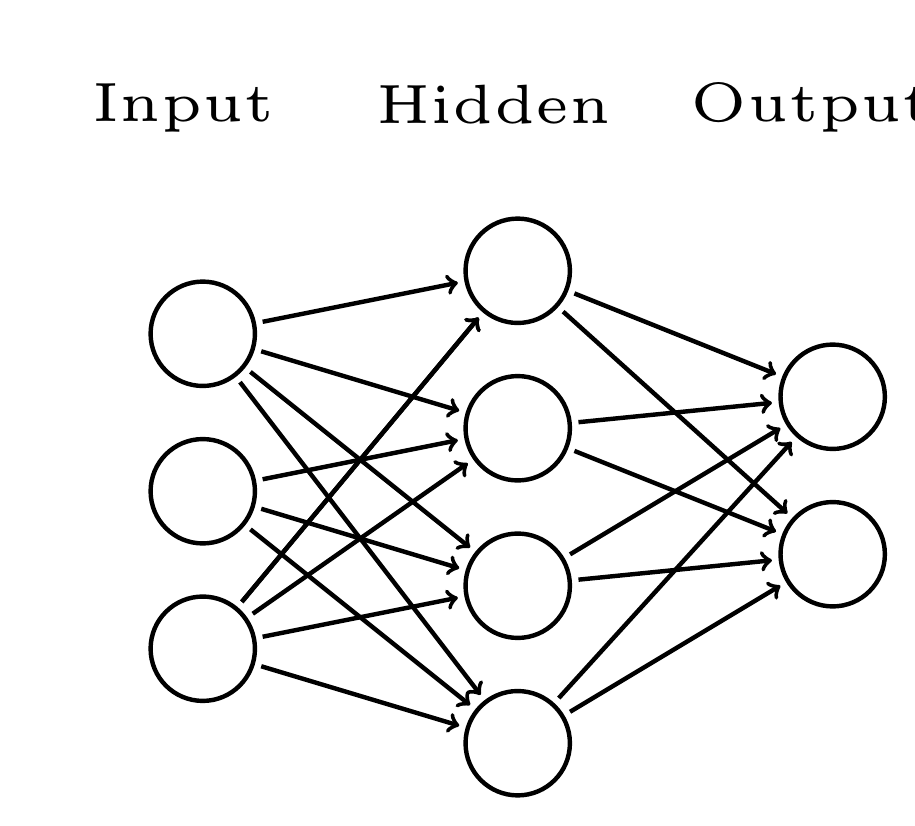
\begin{tikzpicture}[->,ultra thick,scale=4]
      \tikzstyle{every node}=[draw,shape=circle,scale=4]

      \node[draw=none,anchor=north,text width=0.1cm,font=\tiny] (input) at (-0.3,3.5) {Input};
      \node (v0) at (0,1.5) {};
      \node (v1) at (0,2) {};
      \node (v2) at (0,2.5) {};

      \node[draw=none,anchor=north,text width=0.1cm,font=\tiny] (input) at (0.6,3.5) {Hidden};
      \node (h0) at (1,1.2) {};
      \node (h1) at (1,1.7) {};
      \node (h2) at (1,2.2) {};
      \node (h3) at (1,2.7) {};

      \node[draw=none,anchor=north,text width=0.1cm,font=\tiny] (input) at (1.6,3.5) {Output};

      \node (o0) at (2,1.8) {};
      \node (o1) at (2,2.3) {};

      \draw (v0) -- (h0);
      \draw (v0) -- (h1);
      \draw (v0) -- (h2);
      \draw (v0) -- (h3);

      \draw (v1) -- (h0);
      \draw (v1) -- (h1);
      \draw (v1) -- (h2);
      \draw (v0) -- (h3);

      \draw (v2) -- (h0);
      \draw (v2) -- (h1);
      \draw (v2) -- (h2);
      \draw (v2) -- (h3);

      \draw (h0) -- (o0);
      \draw (h0) -- (o1);

      \draw (h1) -- (o0);
      \draw (h1) -- (o1);

      \draw (h2) -- (o0);
      \draw (h2) -- (o1);

      \draw (h3) -- (o0);
      \draw (h3) -- (o1);

    \end{tikzpicture}
  }
  \caption{A fully connected, feed-forward, artificial neural network with 3 input, 4 hidden and 2 output nodes.}
  \label{fig:ann}
\end{figure}

There are several ways to train an ANN, but the most common is to use an algorithm called \textit{backpropagation} to perform supervised learning.  The \textit{backpropagation} algorithm is so named because it propagates an error signal backward (from the output nodes toward the input nodes) through the network to assign blame and update connection weights.

Backpropagation can take a long time to converge to a solution, which may be a local optima and not a global one.  The computational complexity of backpropagation means that it can get prohibitively expensive to train large networks.  ANNs also typically grow in width rather than depth, when the model increases in complexity.  The reason for this is twofold:

\begin{enumerate}
\item Adding a new layer, of same size, adds a lot more connections.  In a fully connected, feed-forward, network adding another layer of N nodes will create an additional $N^2$ connections, whereas adding another node only adds $N$ new connections.
\item It is hard to meaningfully propagate an error signal through a very deep network.  Intuitively this makes sense, because as the network grows in depth it gets harder and harder to assign blame for a bad result.
\end{enumerate}

In \cite{bengio09} Bengio makes a convincing case for why deep architectures are preferable to shallow ones.  The key point being that shallow networks are unable to efficiently encode certain functions.  These function are what the author calls \textit{highly varying functions}: functions where a piecewise-linear approximation of the function would require a large number of pieces.  In general this puts traditional ANNs at a disadvantage, and particularly so the ones being trained with backpropagation.

\section{Restricted Boltzman Machines}

A Boltzman machine (BM) is a fully connected network of neuron-like units.  The connections are bidirectional and a stochastic process is used to determine whether a unit is on or not.  The number of connections in a BM makes them rather slow to train.  However, there exists an efficient learning algorithm\cite{hinton06} for a restricted BM (RBM): a BM where intra-layer connections are disallowed.

\begin{figure}[htb]
  \centering
  \scalebox{0.5}
  {
    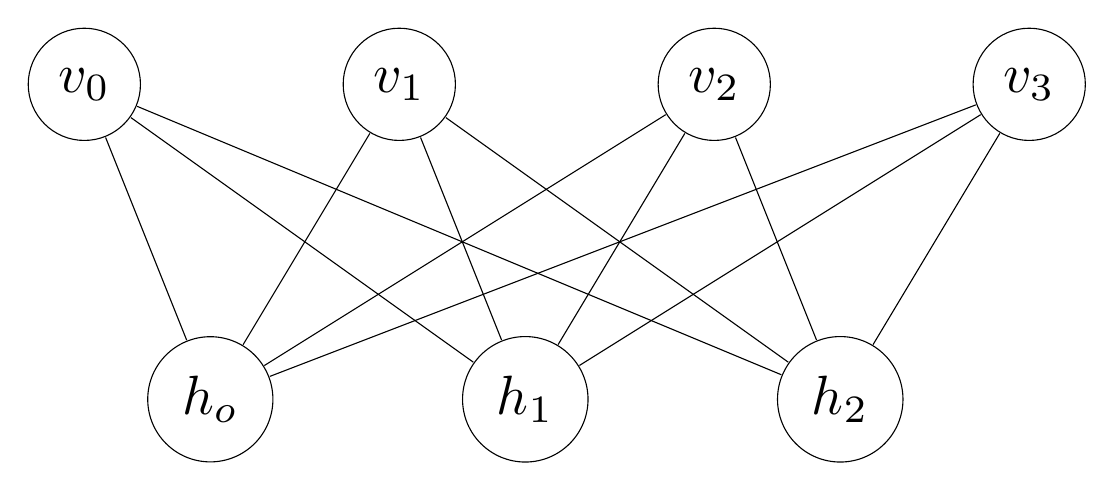
\begin{tikzpicture}[scale=4]
      \tikzstyle{every node}=[draw,shape=circle,scale=2]
      \node (h0) at (0.4,0) {$h_o$};
      \node (h1) at (1.4,0) {$h_1$};
      \node (h2) at (2.4,0) {$h_2$};

      \node (v0) at (0,1) {$v_0$};
      \node (v1) at (1,1) {$v_1$};
      \node (v2) at (2,1) {$v_2$};
      \node (v3) at (3,1) {$v_3$};

      \draw (v0) -- (h0);
      \draw (v0) -- (h1);
      \draw (v0) -- (h2);

      \draw (v1) -- (h0);
      \draw (v1) -- (h1);
      \draw (v1) -- (h2);

      \draw (v2) -- (h0);
      \draw (v2) -- (h1);
      \draw (v2) -- (h2);

      \draw (v3) -- (h0);
      \draw (v3) -- (h1);
      \draw (v3) -- (h2);
    \end{tikzpicture}
  }
  \label{fig:rbm}
  \caption{RBM with 4 visible and 3 hidden nodes.}
\end{figure}

Although RBMs might be unable to efficiently represent some distributions that can be compactly represented by a BM, it can be shown that an RBM, given enough hidden units, can represent any distribution\cite{le08}.  In addition, unless the RBM already perfectly models the training distribution, adding another hidden node (with correct weights and biases) always improves the model\cite{le08}.

The restricted Boltzman machine is so named because the energy metaphor is borrowed from physics.  In physics the Boltzman distribution describes the fractional number of particles occupying a set of states with a given energy and temperature.  In our case each input vector has a corresponding energy level.  During training this multi-dimensional energy landscape will be excavated to create ravines with clusters of training cases.  If the task is handwritten digit recognition then each digit class will map to a ravine in the energy landscape.  As in physics, the lower energy states are the most stable.

An RBM is not limited to doing discrimination, it is a generative model.  This means that the trained model can show its user what it believes in.  Sampling from the model is done using a process called Gibbs sampling.  To perform Gibbs sampling we clamp an input on the visible layer which activates the hidden layer.  The hidden layer activation is in turn used to activate the visible layer.  If we repeat this process sufficiently many times it will converge.  We can start the process off by sending in an instance of training data, e.g an example of a handwritten 9, this will seed the model in a favorable way and the process of Gibbs sampling will converge quicker.  In practice this means starting the model off inside the energy ravine containing known examples of other 9s and then having the model wander around until it settles on a state.  If we start the sampling process off with a random input vector, the process will take longer to converge and we are unable to affect which area of the energy landscape is explored to find a stable energy state.

\section{Autoencoders}

 An autoencoder takes an input $\mathbf{x} \in [0,1]^d$ and maps it--the encoding part--to a representation in the hidden units, $\mathbf{y} \in [0,1]^{d'}$, through a deterministic mapping:
 $\mathbf{y} = s(\mathbf{W}\mathbf{x} + \mathbf{b})$ where $s$ is a non-linear function, e.g. a function from the Sigmoid family.

 The latent representation $\mathbf{y}$, or \textit{code}, is then mapped back--the decoding part--into a reconstruction $\mathbf{z} = s(\mathbf{W'}\mathbf{y} + \mathbf{b'})$.  The transformation is completely analogue with the encoding step and $\mathbf{z}$ has the same shape as $\mathbf{x}$.  Note that ' does not mean that the vectors or matrices are transposed in this context.

Optionally we can let $\mathbf{W'} = \mathbf{W}^T$.  Using this constraint we say that the weights are \textit{tied}.  This same terminology is used for RBMs as well and in that context it means that we are using the same weights for discrimination and generation.

The parameters of the autoencoder $W, b and b'$ are optimized such that the average reconstruction error is minimized.  One way to do this would be to use the \textit{squared error} to guide the weight changes.

\begin{figure}[htb]
  \centering
  \scalebox{0.6}
  {
    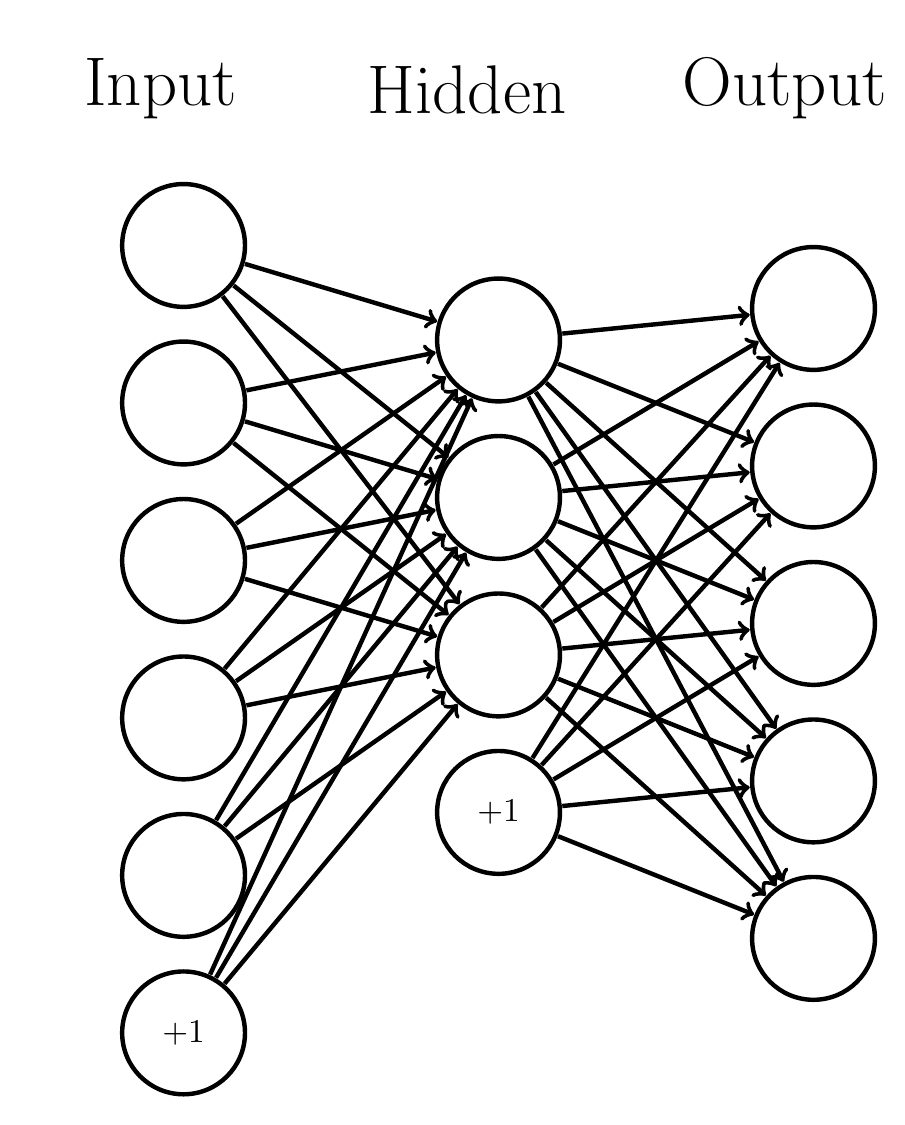
\begin{tikzpicture}[->,ultra thick,scale=4]
      \tikzstyle{every node}=[draw,shape=circle,minimum size=1.3cm,scale=4,text=,scale=0.3]

      \node[draw=none,anchor=north,text width=0.1cm,text=,scale=1,font=\huge] (input) at (-0.3,4.7) {Input}; %
      \node (v0) at (0,1.5) {+1};
      \node (v1) at (0,2) {};
      \node (v2) at (0,2.5) {};
      \node (v3) at (0,3) {};
      \node (v4) at (0,3.5) {};
      \node (v5) at (0,4) {};

      \node[draw=none,anchor=north,text width=0.1cm,text=,scale=1,font=\huge] (input) at (0.6,4.7) {Hidden};
      \node (h0) at (1,2.2) {+1};
      \node (h1) at (1,2.7) {};
      \node (h2) at (1,3.2) {};
      \node (h3) at (1,3.7) {};

      \node[draw=none,anchor=north,text width=0.1cm,text=,scale=1,font=\huge] (input) at (1.6,4.7) {Output};

      \node (o0) at (2,1.8) {};
      \node (o1) at (2,2.3) {};
      \node (o2) at (2,2.8) {};
      \node (o3) at (2,3.3) {};
      \node (o4) at (2,3.8) {};

      \draw (v0) -- (h1);
      \draw (v0) -- (h2);
      \draw (v0) -- (h3);

      \draw (v1) -- (h1);
      \draw (v1) -- (h2);
      \draw (v1) -- (h3);

      \draw (v2) -- (h1);
      \draw (v2) -- (h2);
      \draw (v2) -- (h3);

      \draw (v3) -- (h1);
      \draw (v3) -- (h2);
      \draw (v3) -- (h3);

      \draw (v4) -- (h1);
      \draw (v4) -- (h2);
      \draw (v4) -- (h3);

      \draw (v5) -- (h1);
      \draw (v5) -- (h2);
      \draw (v5) -- (h3);

      \draw (h0) -- (o0);
      \draw (h0) -- (o1);
      \draw (h0) -- (o2);
      \draw (h0) -- (o3);
      \draw (h0) -- (o4);

      \draw (h1) -- (o0);
      \draw (h1) -- (o1);
      \draw (h1) -- (o2);
      \draw (h1) -- (o3);
      \draw (h1) -- (o4);

      \draw (h2) -- (o0);
      \draw (h2) -- (o1);
      \draw (h2) -- (o2);
      \draw (h2) -- (o3);
      \draw (h2) -- (o4);

      \draw (h3) -- (o0);
      \draw (h3) -- (o1);
      \draw (h3) -- (o2);
      \draw (h3) -- (o3);
      \draw (h3) -- (o4);

    \end{tikzpicture}
  }
  \caption{An autoencoder with 5 input, 3 hidden, and 5 output nodes.  Bias nodes are included in the input and hidden layer.}
  \label{fig:ae}
\end{figure}

The gist of it all is that the autoencoder does its best to replicate the input.  The autoencoder drawn in \ref{fig:ae} is perhaps the most common form, where the layer(s) between the input and output layer has a lower dimension.  This will force the autoencoder to learn a compressed representation of the input vector, which it then uses to create the output.  Intuitively, one would think that if the intermediary representation was of the same, or higher dimension, the autoencoder would simply learn the identity function.  Bengio et al. tackled this question in \cite{bengio07} and found that ``layers with non-decreasing layer sizes generalize well'', they speculate that this might be explained by their use of stochastic gradient decent and weight decay.  In other words in the general case, we might risk learning the identity function.

\subsection{Denoising Autoencoders}

The denoising autoencoder is a stochastic version of the autoencoder.  Stochastic because the input is corrupted through some stochastic process.  The non-corrupted input is however used as a target for reconstruction.  The corruption process is performed by setting some, but not more than half, of the inputs to zero.  The denoising autoencoder is thus trying to perform two tasks:
\begin{enumerate}
\item Encode the input
\item Undo the effect of corruption
\end{enumerate}

The motivation behind the denoising autoencoder is to attempt to answer the question ``what properties should we demand of a good representation?''  Many come to mind, but the one investigated in \cite{bengio07} is ``robustness to partial destruction of the input''.  For high dimensional inputs, with redundant information (like in images), the representation is likely to depend on many factors along many dimensions and therefore likely be recoverable from partial observations.  The obvious example, mentioned in the paper, is our human ability to recognize objects which are partially covered up or corrupted in images.

\section{Deep Belief Networks}

\subsection{Using RBMs}

A deep belief network (DBN) can be created by stacking multiple RBMs.  When the input vector is processed by the first RBM its output is a new representation of the data.  This new representation can then be used as input to the RBM in the layer above.  The hope is that each RBM is better able to represent the data, by creating useful abstractions or simply removing noise.  In \cite{hinton06} Hinton shows that adding more layers in a DBN will always improve the model.  The use of the \textit{contrastive divergence} learning algorithm voids this guarantee, but it increases our confidence in the method to know that we can always improve the model by being patient enough in training each layer.

The way to train a DBN is to use a greedy layer-wise training algorithm.  Each layer, consisting of one RBM, is trained before we move on to train the next one.  By freezing the weights after we're done training each RBM we miss out on any positive effect that might be had by the coordinated tuning of weights in two, or more, adjacent layers.  One way to overcome this inefficiency of the greedy training approach is to fine-tune the network after the greedy training phase is done.  Fine-tuning can be done using the well-known backpropagation algorithm, or some other algorithm for gradient decent.  By seeding the backpropagation algorithm with a promising state the following problems encountered using backpropagation in deep networks are solved\cite{hinton06reducing}:
\begin{enumerate}
\item If the initial weights are small the gradients in the earlier layers will be tiny and weight changes ineffectual.
\item If the initial weights are large the network typically gets stuck in poor local minima.
\end{enumerate}

When the initial weights are just right, gradient decent works quite well.

\subsection{Using autoencoders}

A deep belief network can also be created by stacking multiple (denoising) autoencoders.  The process is entirely analogous to the situation with RBMs.  First the network is trained unsupervised pre-training and then fine-tuned using an algorithm like backpropagation.  In \cite{bengio07} DBN using stacked denoising autoencoders were found to perform as good, or better, than DBN networks of stacked RBMs, on the MNIST dataset.

\section{Convolutional Neural Networks}

\subsection{Neocognitron}

\subsection{Multi-column deep neural network}

\subsection{Convolutional Deep Belief Network}


\section{Conclusion}

\appendix

\section{Glossary}



\bibliographystyle{plain}
\bibliography{references}

\end{document}
